\documentclass[UTF8]{ctexart}

\newcommand\subtitle[1]{{\small #1}}

\title{\textbf{2024-2025学年第2学期}\\ \textbf{C++课程作业}\\ \subtitle{仿QQ的聊天程序} \\ \small 班级:24-1} % 在这里直接添加班级信息
\author{\textbf{成员:}\\ \underline{2410120025 郭警豪} \\ \underline{2410120034 陈晓豪}
}
\date{\today}

\usepackage{graphicx} %插入图片的宏包
\usepackage{float} %设置图片浮动位置的宏包
\usepackage{subfigure} %插入多图时用子图显示的宏包

\usepackage{listings}
\usepackage{ctex}
\usepackage{xcolor}
\lstset{
	language=C++,                  % 代码语言
	basicstyle=\ttfamily\small,     % 代码字体
	numbers=left,                   % 行号位置
	numberstyle=\scriptsize\color{gray}, % 行号字体大小和颜色
	stepnumber=1,                   % 行号步长
	numbersep=5pt,                  % 行号与代码的距离
	backgroundcolor=\color{gray!10}, % 背景颜色
	showspaces=false,               % 是否显示空格
	showstringspaces=false,         % 是否显示字符串中的空格
	showtabs=false,                 % 是否显示制表符
	frame=single,                   % 代码边框
	tabsize=2,                      % 制表符宽度
	captionpos=b,                   % 标题位置
	breaklines=true,                % 自动换行
	breakatwhitespace=false,        % 在空白处自动换行
	escapeinside={\%*}{*)},         % 转义字符
	extendedchars=false,            % 非ASCII字符
	linewidth=0.9\textwidth,         % 代码宽度
	aboveskip=3mm,                  % 上方间距
	belowskip=3mm,                  % 下方间距
	columns=fullflexible,            % 列宽自适应
	keepspaces=true,                % 保留空格
	showlines=true,                 % 显示所有行
	keywordstyle=\color{blue},       % 关键字样式
	commentstyle=\color{green},      % 注释样式
	stringstyle=\color{red},        % 字符串样式
	morekeywords={class,template},   % 额外的关键字
}
\usepackage{ragged2e}
\begin{document}
\maketitle
\tableofcontents
\newpage

\section{程序说明}

\RaggedRight % 开始左对齐
\textbf{我们小组开发了一个仿QQ的聊天程序,主要实现了以下功能:}
\begin{itemize}
	\item 用户注册与登录:用户可以通过输入用户名和密码进行注册和登录。
	\item 好友管理:用户可以搜索其他用户并添加为好友,查看好友列表,同意或拒绝好友申请。
	\item 聊天功能:用户可以与好友进行单聊,发送和接收文本消息,并查看历史聊天记录。
\end{itemize}
\textbf{该程序使用Qt框架开发客户端界面,Sqlite数据库存储用户信息和聊天记录,通过Socket实现客户端与服务端的通信。}

\section{小组分工}
\textbf{郭警豪}
\begin{itemize}
	\item 注册与登录功能的实现
	\item 好友功能的实现
	\item 远程服务器的搭建
\end{itemize}
 \textbf{陈晓豪}
\begin{itemize}
	\item 聊天界面的开发
	\item 聊天记录本地化的实现
\end{itemize}
	

\section{程序分析}
\subsection{功能需求}
\begin{itemize}
	\item 用户管理**:支持用户注册、登录,存储用户信息。
	\item 好友管理**:支持搜索用户、添加好友、查看好友列表、处理好友申请。
	\item 聊天功能**:支持单聊,发送和接收消息,查看历史消息。
\end{itemize}	
\subsection{性能需求}
\begin{itemize}
	\item 响应速度:用户操作(如登录、发送消息)应在短时间内得到响应。
	\item 数据存储:用户信息和聊天记录需安全存储,支持历史消息查询。
	\item 并发处理:支持多个用户同时在线,处理并发通信。
\end{itemize}
	
\section{程序设计}
\subsection{设计思路}
\begin{itemize}
	\item 客户端:使用Qt框架开发图形用户界面,实现用户交互功能。
	\item 服务端:处理客户端请求,与数据库交互,存储和查询数据。
	\item 通信:通过Socket实现客户端与服务端的通信,传输JSON格式的数据。
\end{itemize}
\subsection{数据库设计}
\begin{figure}[h]
	\centering
	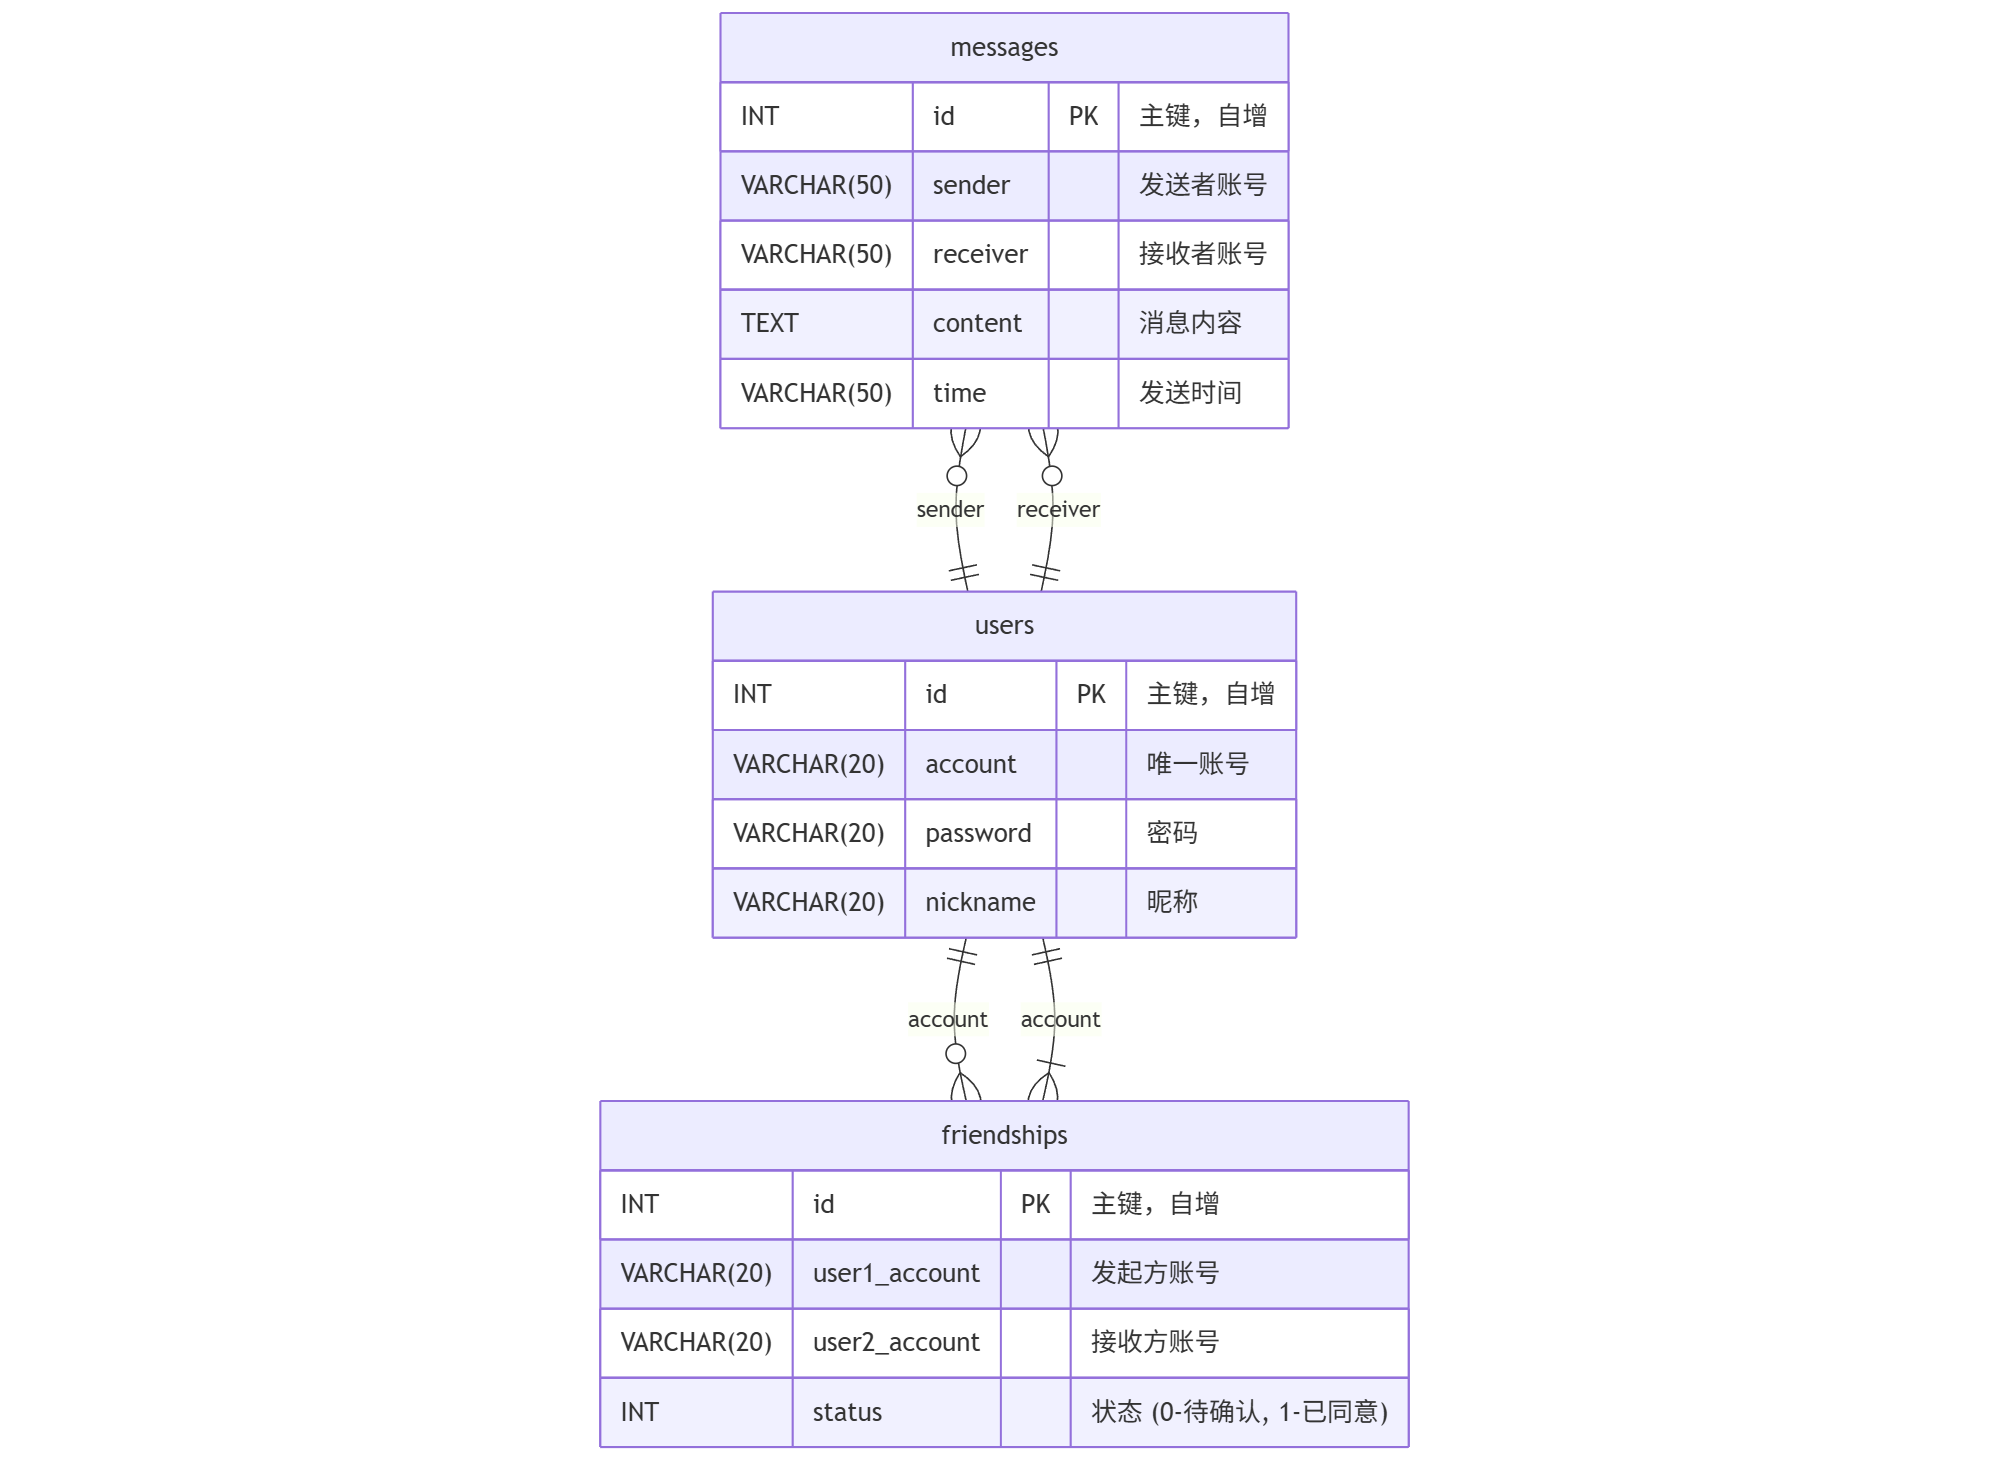
\includegraphics[width=1\textwidth]{sql}
	\caption{数据库设计图(待完善)}
\end{figure}
\subsubsection{用户表(\texttt{users})}
\begin{table}[h]
	\centering
	\begin{tabular}{|c|c|c|}
		\hline
		字段名 & 数据类型 & 描述 \\
		\hline
		\texttt{account} & \texttt{VARCHAR(20)} & 用户账号(主键) \\
		\texttt{password} & \texttt{VARCHAR(50)} & 密码 \\
		\texttt{nickname} & \texttt{VARCHAR(50)} & 昵称 \\
		\hline
	\end{tabular}
	\caption{用户表(\texttt{users})结构}
	\label{tab:users}
\end{table}

\subsubsection{好友关系表(\texttt{friendships})}
\begin{table}[h]
	\centering
	\begin{tabular}{|c|c|c|}
		\hline
		字段名 & 数据类型 & 描述 \\
		\hline
		\texttt{user1\_account} & \texttt{VARCHAR(20)} & 用户1账号 \\
		\texttt{user2\_account} & \texttt{VARCHAR(20)} & 用户2账号 \\
		\texttt{status} & \texttt{INT} & 好友状态(0:申请中,1:已通过) \\
		\hline
	\end{tabular}
	\caption{好友关系表(\texttt{friendships})结构}
	\label{tab:friendships}
\end{table}

\subsubsection{消息表(\texttt{messages})}
\begin{table}[h]
	\centering
	\begin{tabular}{|c|c|c|}
		\hline
		字段名 & 数据类型 & 描述 \\
		\hline
		\texttt{sender} & \texttt{VARCHAR(20)} & 发送者账号 \\
		\texttt{receiver} & \texttt{VARCHAR(20)} & 接收者账号 \\
		\texttt{content} & \texttt{TEXT} & 消息内容 \\
		\texttt{time} & \texttt{DATETIME} & 发送时间 \\
		\hline
	\end{tabular}
	\caption{消息表(\texttt{messages})结构}
	\label{tab:messages}
\end{table}
\subsection{类与函数设计}
\begin{figure}[h]
	\centering
	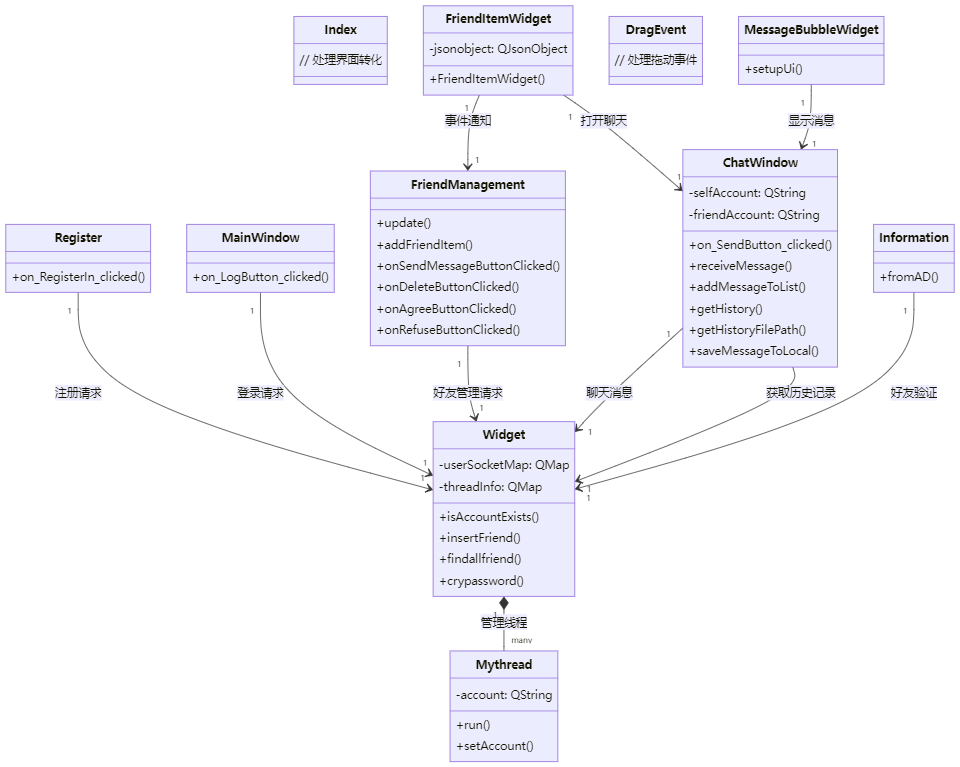
\includegraphics[width=0.4\textwidth]{class}
	\caption{类图(待完善)}
\end{figure}
\begin{itemize}
	\item \textbf{客户端}
	\begin{itemize}
		\item \texttt{Register}:注册界面类,处理用户注册逻辑。
		\item \texttt{MainWindow}:主窗口类,处理用户登录。
		\item \texttt{ChatWindow}:聊天窗口类,处理消息发送和接收。
		\item \texttt{Index}:主界面类,处理界面转化。
		\item \texttt{FriendManagement}:好友管理界面类,处理好友管理。
		\item \texttt{FriendItemWidget}:好友元素类,用于好友显示。
		\item \texttt{DragEvent}:拖动事件类,处理拖动事件。
		\item \texttt{Information}:信息类,处理用户信息显示与发送好友申请。
		\item \texttt{MessageBubbleWidget}:消息气泡类,处理聊天信息的显示。
	\end{itemize}
	\item \textbf{服务端}
	\begin{itemize}
		\item \texttt{Widget}:服务端主类,处理客户端请求,与数据库交互。
		\item \texttt{Mythread}:线程类,用于实现多线程。
	\end{itemize}
\end{itemize}
\section{开发环境}
\begin{itemize}
	\item QT 6.9.0(windows)
	\item Sqlite 3.50.1(windows)
	\item QT 5.15.13(Ubuntu 24.04 64位)
	\item Sqlite 3.45.1(Ubuntu 24.04 64位)
\end{itemize}
\section{程序实现}
\subsection{注册与登录}
\subsubsection{注册}
用户输入昵称和密码后使用Tcp协议传输到服务端,服务端接受到后随机生成一段8到13位的随机数,对接受的密码依次使用Md5,Sha256,Real
Sha3\textunderscore384加密,服务端将账号信息插入数据库中,将账号发回给服务端。
\subsubsection{登录}
用户输入账号和密码,传输到服务端处,服务端在数据库中查找相应账号,与接受到的密码进行比对,服务端将将校验结果发送给客户端,客户端根据接受到的结果判断是否进入Index界面。
\subsubsection{好友申请}
客户端点击Index界面右上角的+号,点击添加好友/群按钮,进入Add
Friend界面,在搜索栏处使用关键词搜索,将关键词发送给服务端,服务端将关键词作为账号和昵称在数据库中查询,并将查询结果发送给客户端,客户端将接受到的结果显示到resultlistView上。用户双击相应条目后进入Informatio
n界面,客户端发出checkFriend请求,客户端检查发送者与被查看者的关系,将结果发送给客户端,客户端根据结果确定按钮的文字,若检查结果is not friend,按钮文字发送好友申请,否则为发送消息。用户点击申请好友按钮后,向服务端发送好友申请,服务端将好友关系插入数据库中,status置为0,代表好友申请未同意。
\subsection{好友管理}
客户端发送upadte请求,服务端查询数据库中所有与此账户有关的好友关系,将好友账号,昵称与status返回,客户端根据返回结果显示相应信息,status为0时显示同意与拒绝按钮,status为1时显示发送消息与删除好友按钮。客户端点击相应按钮后,向服务端发送相应请求,服务端对其请求进行相应处理,并向客户端发送新的好友关系结果,客户端据此更新显示。
\subsection{聊天}
待陈晓豪上传
\subsection{聊天记录的本地存储}
待陈晓豪上传
\section{程序测试}
\textbf{测试账号:}
\begin{itemize}
	\item admin 509919938 root (此账号位于远程服务器上)
\end{itemize}
暂未完全实现
\section{程序部署}
服务端部署在阿里云上,服务器系统使用Ubuntu 24.04 64位,在服务器上安装Sqlite与Qt运行环境,使用Makefile编译程序。同时使用Qt的winde
ployqt命令打包了可在windows下运行的客户端与服务端。
\section*{9 经验总结}

在本次C++课程作业中,我们小组成功开发了一个仿QQ的聊天程序。通过这个项目,我们不仅加深了对C++编程语言的理解,还学习了如何使用Qt框架进行图形用户界面的开发,以及如何通过Socket实现客户端与服务端的通信。以下是我们在开发过程中的一些经验和总结:

\subsection*{技术学习}

\begin{itemize}
	\item \textbf{C++编程}:通过实际项目,我们更加熟悉了C++的基本语法和高级特性,如类和对象、继承和多态等。
	\item \textbf{Qt框架}:我们学习了如何使用Qt框架进行界面设计和事件处理,这极大地提高了我们的界面开发效率。
	\item \textbf{数据库操作}:通过使用Sqlite数据库,我们掌握了基本的数据库操作,包括数据的增删改查。
	\item \textbf{网络编程}:我们学习了如何使用Socket进行网络通信,实现了客户端与服务端的数据交换。
\end{itemize}

\subsection*{项目管理}

\begin{itemize}
	\item \textbf{分工合作}:我们小组明确分工,每位成员负责不同的模块,这不仅提高了开发效率,也确保了项目的顺利进行。
	\item \textbf{版本控制}:使用Git进行版本控制,确保了代码的安全性和可追溯性,方便了团队协作。
	\item \textbf{定期会议}:我们定期举行小组会议,讨论项目进度和遇到的问题,及时调整开发计划。
\end{itemize}

\subsection*{问题解决}

\begin{itemize}
	\item \textbf{调试与测试}:在开发过程中,我们遇到了各种问题,通过调试和测试,我们学会了如何定位和解决问题。
	\item \textbf{性能优化}:针对程序的性能瓶颈,我们进行了优化,提高了程序的响应速度和数据处理能力。
	\item \textbf{安全问题}:我们注意到了程序的安全性,对用户密码进行了加密处理,保护了用户数据的安全。
\end{itemize}

\subsection*{未来展望}

\begin{itemize}
	\item \textbf{功能扩展}:我们计划在未来的版本中增加更多功能,如群聊、文件传输等,以提高程序的实用性。
	\item \textbf{用户体验}:我们将继续优化用户界面和交互设计,提升用户体验。
	\item \textbf{技术探索}:我们希望探索更多的技术,如使用更高级的数据库系统,或者尝试使用其他编程语言进行开发。
\end{itemize}

通过这次课程作业,我们不仅提升了自己的技术能力,也学会了如何进行团队合作和项目管理。我们相信这些经验将对我们未来的学习和工作产生积极的影响。
\appendix
\section{重要代码展示}
\begin{lstlisting}[language=C++, caption=服务端接受信息并处理]
void Server ::newMessageReciver(QByteArray byte,Mythread *currentThread){
	QTcpSocket *socket =currentThread->getSocket();
	
	QJsonObject response;
	
	QJsonDocument receiverdocument = QJsonDocument::fromJson(byte);
	
	qDebug()<<"接受的信息:"<<receiverdocument;
	if(!receiverdocument.isNull()&&receiverdocument.isObject()){
		QJsonObject receiverjsonObject =receiverdocument.object();
		QString type =receiverjsonObject.value("type").toString();
		qDebug()<<receiverjsonObject;
		if(type=="login"){
			QString account = receiverjsonObject.value("account").toString();
			QString password = receiverjsonObject.value("password").toString();
			password=crypassword(password);
			QSqlQuery query;
			query.prepare("SELECT * FROM users WHERE account = :account");
			query.bindValue(":account", account);
			if(query.exec()){
				response["type"] = "login_response";
				if(query.next()){
					int storeId = query.value(0).toInt();
					QString storeAccount = query.value(1).toString();
					QString storePassword = query.value(2).toString();
					QString snickName = query.value(3).toString();
					
					QJsonObject jsonObject;
					jsonObject["id"] = storeId;
					jsonObject["account"] = storeAccount;
					jsonObject["nickname"] = snickName;
					if(storePassword==password){
						
						response["status"] = "success";
						response["message"] = "Login successful";
						
						response["account"]=storeAccount;
						response["nickname"]=snickName;
						response["id"]=storeId;
						currentThread->setAccount(storeAccount);
						threadInfo[storeAccount]=currentThread;
						userSocketMap[storeAccount] = socket;
					}else{
						
						response["status"] = "failure";
						response["message"] = "Incorrect password";
					}
				}else{
					
					response["status"] = "failure";
					response["message"] = "Account not found";
				}
			}
			
		}else if(type=="register"){
			
			QString account = QString::number(QRandomGenerator::global()->bounded(static_cast<double>(1000000000LL)) + 10000000, 'f', 0);
			while(isAccountExists(account)){
				QString account = QString::number(QRandomGenerator::global()->bounded(static_cast<double>(1000000000LL)) + 10000000, 'f', 0);
			}
			QString nickname =receiverjsonObject.value("nickname").toString();
			QString password = receiverjsonObject.value("password").toString();
			password=crypassword(password);
			
			QSqlQuery query;
			query.prepare("INSERT INTO users (account, password, nickname) VALUES (?, ?, ?)");
			query.addBindValue(account);
			query.addBindValue(password);
			query.addBindValue(nickname);
			
			qDebug() << "SQL Query:" << query.lastQuery();
			qDebug() << "Bound Parameters: account=" << account << ", password=" << password << ", nickname=" << nickname;
			
			response["type"] = "register_response";
			if (query.exec()) {
				
				QString successMessage = QString("Registration successful: Account: %1, Nickname: %2").arg(account, nickname);
				qDebug()<<successMessage;
				
				
				response["status"] = "success";
				response["message"] = "Registration successful";
				response["account"] = account; // 返回生成的账号
				
				
				insertFriend(account,account,1);
			} else {
				QString errorMessage = QString("Registration failed: Error: %1")
				.arg(query.lastError().text());
				qDebug()<<errorMessage;
				response["type"] = "register_response";
				response["status"] = "failure";
				response["message"] = query.lastError().text();
			}
			
		}else if(type=="addFriend_search"){
			QString message=receiverjsonObject.value("message").toString();
			
			QSqlQuery query_n;
			query_n.prepare("SELECT account,nickname FROM users WHERE nickname = :message");
			query_n.bindValue(":message", message);
			QSqlQuery query_a;
			query_a.prepare("SELECT account,nickname FROM users WHERE account = :message");
			query_a.bindValue(":message", message);
			QJsonArray usersArray;
			if(query_n.exec()){
				while(query_n.next()){
					
					QString account = query_n.value("account").toString();
					QString nickname = query_n.value("nickname").toString();
					
					
					QJsonObject userObject;
					userObject["account"] = account;
					userObject["nickname"] = nickname;
					
					
					usersArray.append(userObject);
				}
			}
			if (query_a.exec()) {
				while (query_a.next()) {
					
					QString account = query_a.value("account").toString();
					QString nickname = query_a.value("nickname").toString();
					
					QJsonObject userObject;
					userObject["account"] = account;
					userObject["nickname"] = nickname;
					
					
					usersArray.append(userObject);
				}
			}
			response["type"]="addFriend_searcher_reponse";
			response["users"]=usersArray;
		}else if (type == "checkFriend") {
			qDebug() << "checkFriend";
			response["type"] = "checkFriend_response";
			
			QString v_account = receiverjsonObject["v_account"].toString();
			QString account = receiverjsonObject["account"].toString();
			
			QSqlQuery query;
			query.prepare("SELECT COUNT(*) AS is_friend FROM friendships WHERE "
			"(user1_account = :v_account AND user2_account = :account AND status = 1) OR "
			"(user2_account = :v_account AND user1_account = :account AND status = 1);");
			query.bindValue(":v_account", v_account);
			query.bindValue(":account", account);
			
			if (query.exec()) {
				if (query.next()) {
					int is_friend = query.value(0).toInt();
					if (is_friend > 0) {
						response["result"] = "is friend";
					} else {
						response["result"] = "is not friend";
					}
				}
			} else {
				qDebug() << "Query failed:" << query.lastError().text();
			}
		}else if(type=="friend_request"){
			response["type"]="friend_request_response";
			QString v_account=receiverjsonObject["v_account"].toString();
			QString account=receiverjsonObject["account"].toString();
			if(insertFriend(v_account,account,0)){
				response["result"]="insert_successed";
			}else{
				response["result"]="insert_not_successed";
			}
			
			auto it = threadInfo.find(account);
			if (it != threadInfo.end()) {
				qDebug() << account<<"在线";
				Mythread* f_thread = it.value();
				QTcpSocket* f_socket=f_thread->getSocket();
				QJsonObject f_response;
				find(account,f_response);
				sendToClient(f_socket,f_response);
			} else {
				qDebug() << account<<"未在线";
			}
		}else if(type=="update"){
			QString account =receiverjsonObject["account"].toString();
			find(account,response);
		}else if(type=="Agree_the_friend"){
			QString account = receiverjsonObject["account"].toString();
			QString friend_account = receiverjsonObject["friend_account"].toString();
			qDebug() << "account:" << account << "friend_account:" << friend_account;
			QSqlQuery query;
			query.prepare("UPDATE friendships SET status = 1 WHERE user1_account = ? AND user2_account = ?;");
			query.addBindValue(friend_account);
			query.addBindValue(account);
			if (query.exec()) {
				qDebug() << "Agree_the_friend" << query.lastQuery();
				find(account,response);
				
				auto it = threadInfo.find(friend_account);
				if (it != threadInfo.end()) {
					qDebug() << friend_account<<"在线";
					Mythread* f_thread = it.value();
					QTcpSocket* f_socket=f_thread->getSocket();
					QJsonObject f_response;
					find(friend_account,f_response);
					sendToClient(f_socket,f_response);
				} else {
					qDebug() << friend_account<<"未在线";
				}
			} else {
				qDebug() << "Update failed:" << query.lastError().text();
			}
			qDebug() << "Agree_the_friend" << query.lastQuery();
		}else if (type=="Refuse_the_friend"||type=="Delete_the_friend"){
			QString account = receiverjsonObject["account"].toString();
			QString friend_account = receiverjsonObject["friend_account"].toString();
			qDebug() << "account:" << account << "friend_account:" << friend_account;
			
			QSqlQuery query;
			query.prepare("DELETE FROM friendships WHERE user1_account = :friend_account AND user2_account = :account;");
			query.bindValue(":account", account);
			query.bindValue(":friend_account", friend_account);
			
			if (query.exec()) {
				qDebug() << "Delete successful";
				find(account,response);
				
				auto it = threadInfo.find(friend_account);
				if (it != threadInfo.end()) {
					qDebug() << friend_account<<"在线";
					Mythread* f_thread = it.value();
					QTcpSocket* f_socket=f_thread->getSocket();
					QJsonObject f_response;
					find(friend_account,f_response);
					sendToClient(f_socket,f_response);
				} else {
					qDebug() << friend_account<<"未在线";
				}
			} else {
				qDebug() << "Delete failed:" << query.lastError().text();
			}
		}
		else if(type == "chat_message"){
			QString from = receiverjsonObject["from"].toString();
			QString to = receiverjsonObject["to"].toString();
			qDebug() << "to_user:::" << from << to;
			QString content = receiverjsonObject["content"].toString();
			QString time = receiverjsonObject["time"].toString();
			
			QJsonObject chatData;
			chatData["type"] = "chat_message";
			chatData["from"] = from;
			chatData["to"] = to;
			chatData["content"] = content;
			chatData["time"] = time;
			
			QJsonDocument doc(chatData);
			QByteArray data = doc.toJson();
			
			
			QSqlQuery saveChat;
			saveChat.prepare("INSERT INTO messages (sender, receiver, content, time) VALUES (:from, :to, :content, :time)");
			saveChat.bindValue(":from", from);
			saveChat.bindValue(":to", to);
			saveChat.bindValue(":content", content);
			saveChat.bindValue(":time", time);
			
			if (!saveChat.exec()) {
				qDebug() << "Failed to save message:" << saveChat.lastError().text();
			} else {
				qDebug() << "Message saved successfully";
			}
			
			
			if (userSocketMap.contains(to)) {
				userSocketMap[to]->write(data);
				response["status"] = "sent";
			} else {
				response["status"] = "offline";
			}
		}
		else if(type == "get_history") {
			QString a1 = receiverjsonObject["from"].toString();
			QString a2 = receiverjsonObject["to"].toString();
			
			QSqlQuery query;
			query.prepare("SELECT sender, receiver, content, time FROM messages WHERE "
			"(sender = :a1 AND receiver = :a2) OR (sender = :a2 AND receiver = :a1) "
			"ORDER BY time ASC");
			query.bindValue(":a1", a1);
			query.bindValue(":a2", a2);
			
			
			QMap<QString, QString> nicknameMap;
			QSqlQuery nicknameQuery;
			nicknameQuery.prepare("SELECT account, nickname FROM users WHERE account = :a1 OR account = :a2");
			nicknameQuery.bindValue(":a1", a1);
			nicknameQuery.bindValue(":a2", a2);
			if (nicknameQuery.exec()) {
				while (nicknameQuery.next()) {
					QString account = nicknameQuery.value("account").toString();
					QString nickname = nicknameQuery.value("nickname").toString();
					nicknameMap[account] = nickname;
				}
			}
			
			QJsonArray msgArray;
			if (query.exec()) {
				while (query.next()) {
					QString sender = query.value("sender").toString();
					QJsonObject msg;
					msg["name"] = nicknameMap.value(sender, sender);//发送者的名称
					msg["from"] = sender;
					msg["to"] = query.value("receiver").toString();
					msg["content"] = query.value("content").toString();
					msg["time"] = query.value("time").toString();
					msgArray.append(msg);
				}
			}
			
			response["type"] = "get_history_response";
			response["messages"] = msgArray;
			
			
		} else if(type == "create_group") {
			QString groupName = receiverjsonObject["group_name"].toString();
			QString ownerAccount = receiverjsonObject["owner_account"].toString();
			
			
			QSqlQuery query;
			query.prepare("INSERT INTO `groups` (group_name, owner_account) VALUES (:group_name, :owner_account)");
			query.bindValue(":group_name", groupName);
			query.bindValue(":owner_account", ownerAccount);
			
			response["type"] = "create_group_response";
			
			if (query.exec()) {
				qint64 groupId = query.lastInsertId().toLongLong();
				
				
				QSqlQuery addMember;
				addMember.prepare("INSERT INTO group_members (group_id, account, role) VALUES (:group_id, :account, 'owner')");
				addMember.bindValue(":group_id", groupId);
				addMember.bindValue(":account", ownerAccount);
				addMember.exec();
				
				response["status"] = "success";
				response["group_id"] = QString::number(groupId);
				response["message"] = "Group created successfully";
				if (!addMember.exec()) {
					qDebug() << "Failed to add group member:" << addMember.lastError().text();
				} else {
					qDebug() << "Added group member successfully.";
				}
			} else {
				response["status"] = "failure";
				response["message"] = query.lastError().text();
			}
			
		}
		
	}
	sendToClient(socket,response);
}
\end{lstlisting}
\begin{lstlisting}[language=c++,caption=chatwindow的实现]
	#include "chatwindow.h"
	#include "ui_chatwindow.h"
	#include "dragevent.h"
	#include <QFile>
	#include <QDir>
	#include <QDesktopServices>
	ChatWindow::ChatWindow(QTcpSocket *socket, const QString &selfAccount, const QString &friendAccount, const QString &friendName, QWidget *parent)
	: QWidget(parent)
	, ui(new Ui::ChatWindow)
	{
		ui->setupUi(this);
		setWindowFlag(Qt::FramelessWindowHint);
		
		ui->MessageListWidget->setSpacing(5);
		ui->MessageListWidget->setSelectionMode(QAbstractItemView::NoSelection);
		ui->MessageListWidget->setFocusPolicy(Qt::NoFocus);
		ui->MessageListWidget->setVerticalScrollMode(QAbstractItemView::ScrollPerPixel);
		ui->MessageListWidget->setStyleSheet(R"(
		QListWidget {
			background: transparent;
			border: none;
		}
		QListWidget::item {
			background: transparent;
			border: none;
			margin: 0px;
			padding: 0px;
		}
		QListWidget::item:hover {
			background: transparent;
		}
		QListWidget::item:selected {
			background: transparent;
		}
		)");
		ui->EditArea->installEventFilter(this);
		this->installEventFilter(new DragEvent());
		this->socket = socket;
		this->selfAccount = selfAccount;
		this->friendAccount = friendAccount;
		this->friendName = friendName;
		if(selfAccount!=friendName){
			ui->FriendName->setText(friendName);
		}
		qDebug() << "to_user:::" << selfAccount << friendAccount;
		loadHistoryFromLocal();
		getHistory();
		
		connect(ui->close,&QToolButton::clicked,this,&ChatWindow::on_close_triggered);
		connect(ui->SendButton, &QPushButton::clicked, this, &ChatWindow::on_SendButton_clicked);
	}
	bool ChatWindow::eventFilter(QObject *obj, QEvent *event) {
		if (obj == ui->EditArea && event->type() == QEvent::KeyPress) {
			QKeyEvent *keyEvent = static_cast<QKeyEvent*>(event);
			if ((keyEvent->key() == Qt::Key_Enter || keyEvent->key() == Qt::Key_Return) &&
			keyEvent->modifiers() == Qt::NoModifier) {
				emit on_SendButton_clicked();
				return true;
			}
		}
		return QWidget::eventFilter(obj, event);
		ui->EditArea->setFocus();
	}
	
	ChatWindow::~ChatWindow()
	{
		delete ui;
	}
	
	
	
	void ChatWindow::on_SendButton_clicked()
	{
		QString text = ui->EditArea->toPlainText();
		while (!text.isEmpty() && text.endsWith('\n')) {
			text = text.chopped(1);
		}
		if (text.isEmpty()) return;
		
		QJsonObject object;
		object["type"] = "chat_message";
		object["from"] = this->selfAccount;
		object["to"] = this->friendAccount;
		
		object["content"] = text;
		object["time"] = QDateTime::currentDateTime().toString("yyyy-MM-dd HH:mm:ss");
		QByteArray data = QJsonDocument(object).toJson();
		socket->write(data);
		
		QString messageLine =  text;
		addMessageToList(messageLine, "皇帝",true);
		ui->EditArea->clear();
		saveMessageToLocal(object);
	}
	
	void ChatWindow::receiveMessage(const QJsonObject &js) {
		qDebug()<<__func__<<js;
		if (js["from"].toString() == friendAccount) {
			QString time = js["time"].toString();
			QString content = js["content"].toString();
			QString messageLine = content;
			addMessageToList(messageLine, js["name"].toString(),false);
			saveMessageToLocal(js);
		}
	}
	
	void ChatWindow::onReadyRead(QJsonObject jsonobject)
	{
		qDebug() << __func__ << jsonobject;
		qDebug() << "Data arrived";
		
		QString type = jsonobject["type"].toString();
		if (type == "chat_message") {
			receiveMessage(jsonobject);
		}
		else if (type == "get_history_response") {
			QJsonArray history = jsonobject["messages"].toArray();
			for (const QJsonValue &val : history) {
				QJsonObject msg = val.toObject();
				processNewMessage(msg);
			}
		}
	}
	
	
	void ChatWindow::on_close_triggered()
	{
		this->hide();
	}
	
	void ChatWindow::getHistory()
	{
		QJsonObject json;
		json["type"] = "get_history";
		json["from"] = this->selfAccount;
		json["to"] = this->friendAccount;
		QByteArray data = QJsonDocument(json).toJson();
		socket->write(data);
	}
	
	void ChatWindow::addMessageToList(const QString &text, const QString &name, bool isOwnMessage)
	{
		
		QWidget *container = new QWidget;
		QVBoxLayout *layout = new QVBoxLayout(container);
		layout->setSpacing(2);
		layout->setContentsMargins(10, 0, 10, 0);
		
		
		QLabel *nameLabel = new QLabel(name);
		nameLabel->setStyleSheet("color: gray; font-size: 10px;");
		if (isOwnMessage) {
			nameLabel->setAlignment(Qt::AlignRight);
		} else {
			nameLabel->setAlignment(Qt::AlignLeft);
		}
		
		
		MessageBubbleWidget *bubble = new MessageBubbleWidget(text, isOwnMessage);
		
		
		layout->addWidget(nameLabel);
		layout->addWidget(bubble);
		
		
		QListWidgetItem *item = new QListWidgetItem(ui->MessageListWidget);
		item->setSizeHint(container->sizeHint());
		
		ui->MessageListWidget->addItem(item);
		ui->MessageListWidget->setItemWidget(item, container);
		ui->MessageListWidget->scrollToBottom();
	}
	
	QWidget* ChatWindow::createTimeLabel(const QString &time)
	{
		QLabel *label = new QLabel(time);
		label->setAlignment(Qt::AlignCenter);
		label->setStyleSheet("color: gray; font-size: 12px; padding: 5px;");
		
		QWidget *wrapper = new QWidget;
		QHBoxLayout *layout = new QHBoxLayout(wrapper);
		layout->addWidget(label);
		layout->setAlignment(Qt::AlignCenter);
		layout->setContentsMargins(0, 0, 0, 0);
		return wrapper;
	}
	
	QString ChatWindow::getHistoryFilePath() const {
		QString filename = QString("%1_%2.json").arg(selfAccount).arg(friendAccount);
		
		
		QString currentPath = QDir::currentPath();
		QString dirPath = currentPath + "/chat_history";
		QDir dir;
		
		
		if (!dir.exists(dirPath)) {
			qDebug() << "正在创建目录:" << dirPath;
			if (!dir.mkpath(dirPath)) {
				qDebug() << "创建目录失败!";
			}
		}
		
		QString fullPath = dirPath + "/" + filename;
		qDebug() << "create" << fullPath;
		return fullPath;
	}
	
	void ChatWindow::saveMessageToLocal(const QJsonObject &msg) {
		QString filePath = getHistoryFilePath();
		qDebug() << "save" << filePath;
		
		QFile file(filePath);
		QJsonArray historyArray;
		
		
		if (file.exists()) {
			qDebug() << "文件已存在,尝试读取历史记录...";
			if (file.open(QIODevice::ReadOnly)) {
				QByteArray data = file.readAll();
				QJsonDocument doc = QJsonDocument::fromJson(data);
				if (doc.isArray()) {
					historyArray = doc.array();
				}
				file.close();
			}
		}
		
		
		QString messageId = msg["id"].toString();
		if (messageId.isEmpty()) {
			QString content = msg["content"].toString();
			QString time = msg["time"].toString();
			messageId = QString("%1_%2").arg(time).arg(content);
		}
		
		bool exists = false;
		for (const QJsonValue &val : historyArray) {
			QJsonObject existingMsg = val.toObject();
			QString existingId = existingMsg["id"].toString();
			if (existingId.isEmpty()) {
				QString existingContent = existingMsg["content"].toString();
				QString existingTime = existingMsg["time"].toString();
				existingId = QString("%1_%2").arg(existingTime).arg(existingContent);
			}
			if (existingId == messageId) {
				exists = true;
				break;
			}
		}
		
		if (!exists) {
			historyArray.append(msg);
			
			if (file.open(QIODevice::WriteOnly | QIODevice::Truncate)) {
				QJsonDocument doc(historyArray);
				qint64 bytesWritten = file.write(doc.toJson());
				qDebug() << " 写入文件成功,共写入" << bytesWritten << "字节";
				file.close();
			} else {
				qDebug() << " 无法打开文件进行写入:" << file.errorString();
			}
		} else {
			qDebug() << " 消息已存在,未写入文件:" << messageId;
		}
		
	}
	void ChatWindow::loadHistoryFromLocal() {
		QString filePath = getHistoryFilePath();
		qDebug() << "get" << filePath;
		
		QFile file(filePath);
		if (!file.exists()) return;
		
		if (file.open(QIODevice::ReadOnly)) {
			QByteArray data = file.readAll();
			QJsonDocument doc = QJsonDocument::fromJson(data);
			if (doc.isArray()) {
				QJsonArray history = doc.array();
				for (const QJsonValue &val : history) {
					QJsonObject msg = val.toObject();
					processNewMessage(msg);
				}
			}
			file.close();
		}
	}
	
	void ChatWindow::processNewMessage(const QJsonObject &msg) {
		QString messageId = msg["id"].toString();
		if (messageId.isEmpty()) {
			
			QString content = msg["content"].toString();
			QString time = msg["time"].toString();
			messageId = QString("%1_%2").arg(time).arg(content);
		}
		
		if (!messageCache.contains(messageId)) {
			QString sender = msg["from"].toString();
			QString content = msg["content"].toString();
			QString name = msg["name"].toString();
			bool isOwn = (sender == selfAccount);
			
			QDateTime timestamp = QDateTime::fromString(msg["time"].toString(), "yyyy-MM-dd HH:mm:ss");
			
			
			if (lastMessageTime.isNull() ||
			lastMessageTime.date() != timestamp.date() ||
			lastMessageTime.secsTo(timestamp) > TIME_THRESHOLD_SECONDS) {
				QListWidgetItem* item = new QListWidgetItem(ui->MessageListWidget);
				QWidget *timeWidget = createTimeLabel(timestamp.toString("yyyy-MM-dd HH:mm:ss"));
				item->setSizeHint(timeWidget->sizeHint());
				ui->MessageListWidget->addItem(item);
				ui->MessageListWidget->setItemWidget(item, timeWidget);
			}
			
			
			addMessageToList(content, name, isOwn);
			
			
			saveMessageToLocal(msg);
			
			
			messageCache.insert(messageId);
			
			
			lastMessageTime = timestamp;
		} else {
			qDebug() << " 消息已存在,跳过:" << messageId;
		}
	}
\end{lstlisting}
\end{document}
